\documentclass[12pt]{article}
\usepackage[english]{babel}
\usepackage[utf8x]{inputenc}
\usepackage{amsmath}
\usepackage{graphicx}
\usepackage[colorinlistoftodos]{todonotes}
\usepackage{pifont}
\usepackage{subfigure}% Support for small, `sub' figures and tables
\usepackage{float} 
\usepackage{array}
%\usepackage{url}
\usepackage[hyphens]{url} %break url
%\usepackage{xurl}
\usepackage{enumitem}
%\usepackage{biblatex}
\newcommand\tab[1][0.6cm]{\hspace*{#1}}
\usepackage{changepage}
\usepackage[nottoc]{tocbibind}



\usepackage{listings} % code listing
\usepackage{color}

\definecolor{dkgreen}{rgb}{0,0.6,0}
\definecolor{gray}{rgb}{0.5,0.5,0.5}
\definecolor{mauve}{rgb}{0.58,0,0.82}

\lstset{frame=tb,
    language=Java,
    aboveskip=3mm,
    belowskip=3mm,
    showstringspaces=false,
    columns=flexible,
    basicstyle={\scriptsize\ttfamily},
    numbers=none,
    numberstyle=\tiny\color{gray},
    keywordstyle=\color{blue},
    commentstyle=\color{dkgreen},
    stringstyle=\color{mauve},
    breaklines=true,
    breakatwhitespace=true,
    tabsize=3
}


\usepackage{csquotes}


\begin{document}
    
    \begin{titlepage}
        
        \newcommand{\HRule}{\rule{\linewidth}{0.5mm}} % Defines a new command for the horizontal lines, change thickness here
        
        \center % Center everything on the page
        
        %----------------------------------------------------------------------------------------
        %    HEADING SECTIONS
        %----------------------------------------------------------------------------------------
        
        \textsc{\large Central Washington University}\\[1.5cm] % Name of your university/college
        \textsc{\Large Advance Algorithm}\\[0.5cm] % Major heading such as course name
        \textsc{\large Winter 2020}\\[0.5cm] % Minor heading such as course title
        
        %----------------------------------------------------------------------------------------
        %    TITLE SECTION
        %----------------------------------------------------------------------------------------
        
        \HRule \\[0.5cm]
        { \Large \bfseries Title-cased Word Count with MapR}
        \\[0.2cm] % Title of your document
        \HRule \\[0.5cm]
        
        %----------------------------------------------------------------------------------------
        %    AUTHOR SECTION
        %----------------------------------------------------------------------------------------
        
        %\begin{minipage}{0.5\textwidth}
        %    \begin{flushleft} \large
                \emph{Student:}
                %\begin{itemize}
                    \textsc {\large Tin Tan Nguyen} \\			
                 \emph{Email:}   ntin\textsc{@cwu.edu}\\
                %\end{itemize}
        %    \end{flushleft}
        %\end{minipage}
        ~
        %\begin{minipage}{0.45\textwidth}
        %    \begin{flushright} \large
        %        \emph{Professor:} \\
        %        Dr. Szilárd \textsc{VAJDA}\\ % Supervisor's Name
        %        Szilard.Vajda@cwu.edu
        %    \end{flushright}
        %\end{minipage}\\[0.5cm]
        
        % If you don't want a supervisor, uncomment the two lines below and remove the section above
        %\Large \emph{Author:}\\
        %John \textsc{Smith}\\[3cm] % Your name
        
        %----------------------------------------------------------------------------------------
        %    DATE SECTION
        %----------------------------------------------------------------------------------------
        \vspace{2cm}
        {\large \today}\\ % Date, change the \today to a set date if you want to be precise
        
        %----------------------------------------------------------------------------------------
        %    LOGO SECTION
        %----------------------------------------------------------------------------------------
        
        
\includegraphics[width=8cm]{CWU-Logo.png}\\[.5cm] % Include a department/university logo - this will require the graphicx package
        
        %----------------------------------------------------------------------------------------
        
        \vfill % Fill the rest of the page with whitespace
        
    \end{titlepage}
    \begin{itemize}
    \item \textbf{Project description}\\\\
    \tab This project will use the concept of MapReduced to find the frequency of title-cased words in many large text files. For this projects, multiple of text books will be used to test the run time analysis of the algorithm.
    
    \item \textbf{MapR description: }\\\\
    \tab Spawn multiple processes to process divided workloads in parallel in order to optimize run-time execution.  
    \item \textbf{Project planning : }\\\\
    \tab First we need to down load a large text file, preferably books from the internet.\\
    \tab Python multiprocessing Pool package will be used to create parallel processes to read and count separate section of the text file simultaneously. \\
    \tab We will start with 2 threads and go to to 8 threads to see if the run-time get improved as threads are increasing. \\
    \tab We then can compare the run-time of MapR method vs sequential method and observe if there is improvement. 
	\item \textbf{Run-time analysis:} \\
	\tab First we need to process the text files to remove all spaces, lines and special characters in the texts. Then we need to put all the words from the text in a list and then we apply both sequential and MapReduce method to count how many title-cased words. 
	\begin{figure}[H]
    	\centering
    	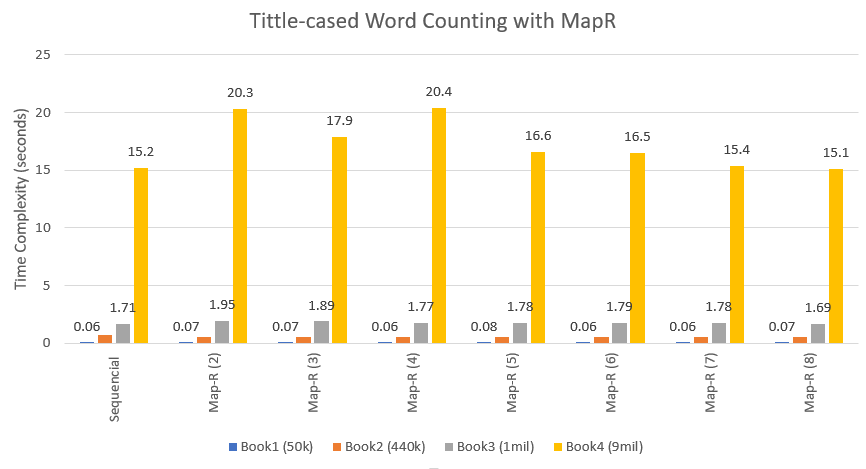
\includegraphics[width=15cm]{analysis1.png}
    	\caption{Time Complexity Analysis} 
    	\label{fig:1}
    \end{figure}
    \tab From looking at the chart above, run-time of sequential method  is a lot better than MapReduce method for smaller and larger samples (<9mil words) because it costs time to create threads and do scheduling. If the sample size is small enough and the task is lightweight, sequential always beat MapReduce method. \\\\
    \tab We can then increase the workload of the task by adding the file processing along with word counting in the main task. This will add more workload for the CPU and this time we should expect to get better run-time of the MapReduce method compare to the sequential method. 
    \begin{figure}[H]
    	\centering
    	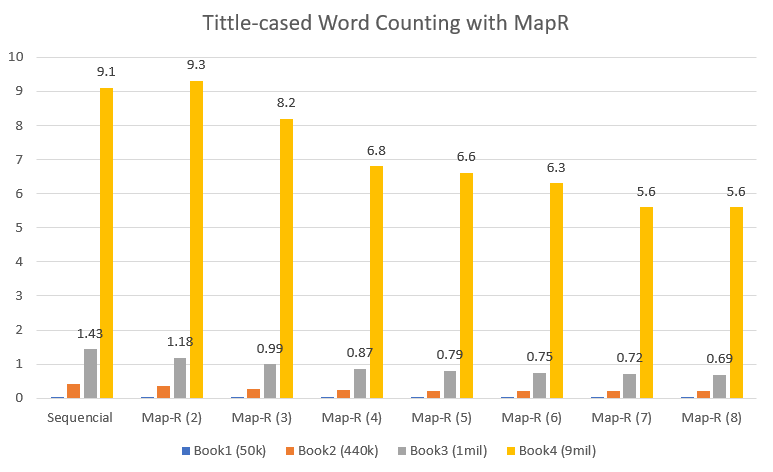
\includegraphics[width=13cm]{analysis2.png}
    	\caption{Time Complexity Analysis} 
    	\label{fig:1}
    \end{figure}   
    \tab As expected, run-time of MapReduce method is much better compare to sequential method in this second experiment just by increasing the workload. For this experiment, MapReduce run-time get saturated when number of processes reach to 7 and the run-time is about 40\% faster compare to sequential method.
	\vfill
	\item \textbf{Python MapR Code: }    
    \begin{figure}[H]
    	\centering
    	\includegraphics[width=13cm]{MapR_code.png}
    	\caption{Python MapR Code} 
    	\label{fig:2}
  	
    \end{figure}
\end{itemize}
\end{document}